%-------------------------
% One-Page CV — Chi-Sheng (Michael) Chen
% Condensed from main.tex. License: MIT
%-------------------------
\documentclass[letterpaper,9pt]{extarticle}

\usepackage{latexsym}
\usepackage[empty]{fullpage}
\usepackage{titlesec}
\usepackage[usenames,dvipsnames]{color}
\usepackage{enumitem}
\usepackage[hidelinks]{hyperref}
\usepackage{fancyhdr}
\usepackage[english]{babel}
\usepackage{tabularx}
\usepackage{graphicx}
\usepackage{fontawesome}

\definecolor{accent}{RGB}{0,51,102}

\pagestyle{fancy}
\fancyhf{}
\fancyfoot{}
\renewcommand{\headrulewidth}{0pt}
\renewcommand{\footrulewidth}{0pt}

% Margins — tight to fit one page
\addtolength{\oddsidemargin}{-0.65in}
\addtolength{\evensidemargin}{-0.65in}
\addtolength{\textwidth}{1.3in}
\addtolength{\topmargin}{-.95in}
\addtolength{\textheight}{1.9in}

\urlstyle{same}
\raggedbottom
\raggedright
\setlength{\tabcolsep}{0in}

% Section formatting
\titleformat{\section}{
  \vspace{-2pt}\scshape\raggedright\normalsize\color{accent}
}{}{0em}{}[\color{accent}\titlerule \vspace{-6pt}]

% Custom commands
\newcommand{\resumeItem}[1]{\item\small{{#1 \vspace{-2pt}}}}

\newcommand{\resumeSubheading}[4]{
  \vspace{-1pt}\item
    \begin{tabular*}{0.98\textwidth}[t]{l@{\extracolsep{\fill}}r}
      \textbf{#1} & #2 \\
      \textit{\small#3} & \textit{\small #4} \\
    \end{tabular*}\vspace{-6pt}
}

\newcommand{\resumeEduHeading}[4]{
  \vspace{-1pt}\item
    \begin{tabular*}{0.98\textwidth}[t]{l@{\extracolsep{\fill}}r}
      \textbf{#1} & #2 \\
      \textit{\small#3} & \textit{\small #4} \\
    \end{tabular*}\vspace{-6pt}
}

\renewcommand\labelitemii{$\vcenter{\hbox{\tiny$\bullet$}}$}

\newcommand{\resumeSubHeadingListStart}{\begin{itemize}[leftmargin=0.12in, label={}]}
\newcommand{\resumeSubHeadingListEnd}{\end{itemize}}
\newcommand{\resumeItemListStart}{\begin{itemize}[leftmargin=0.28in]}
\newcommand{\resumeItemListEnd}{\end{itemize}\vspace{-4pt}}

\begin{document}

%---------- HEADER ----------
\begin{tabular*}{\textwidth}{@{\extracolsep{\fill}} l r}
\begin{minipage}[c]{0.78\textwidth}
  {\Huge \textbf{Chi-Sheng (Michael) Chen}} \\[3pt]
  {\color{accent}\small Physiological Time-Series ML \textbullet\ Biosignal Foundation Models \textbullet\ LLM Agents \textbullet\ Clinical AI} \\[4pt]
  \small
  \faEnvelope\ \href{mailto:m50816m50816@gmail.com}{m50816m50816@gmail.com} \quad
  \faGithub\ \href{https://github.com/ChiShengChen}{ChiShengChen} \\[2pt]
  \faGraduationCap\ \href{https://scholar.google.com.tw/citations?user=5XHD7nkAAAAJ}{Google Scholar} \quad
  \faLinkedin\ \href{https://www.linkedin.com/in/michael-chi-sheng-chen-257359137/}{LinkedIn} \quad
  \faGlobe\ ORCID: 0000-0003-0807-0217
\end{minipage}
&
\begin{minipage}[c]{0.2\textwidth}
  \raggedleft
  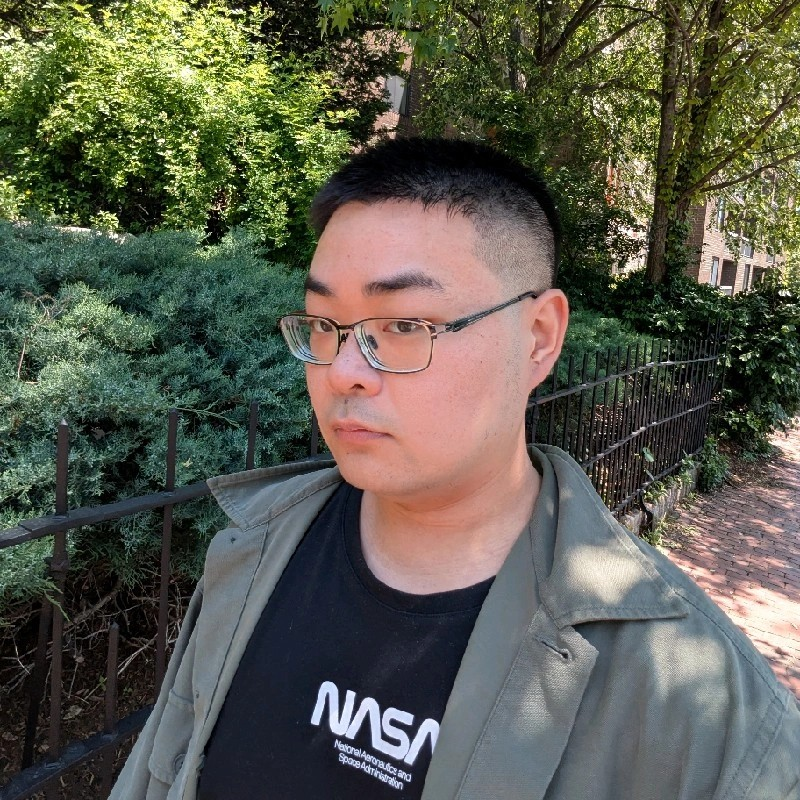
\includegraphics[width=0.95\linewidth]{photo.jpg}
\end{minipage}
\end{tabular*}

\vspace{4pt}
\small Research Affiliate at Harvard Medical School \& BIDMC building interpretable ML for clinical biosignals (EEG, EMS trauma triage) and biosignal foundation models; EEG depression-treatment model in routine clinical use at Taipei VGH. Prior: CTO of Neuro Industry, Digital IC Engineer at MediaTek. Reviewer for NeurIPS/ICML/AAAI/KDD and 35 journals.

%---------- EDUCATION ----------
\section{Education}
\resumeSubHeadingListStart
  \resumeEduHeading
    {National Taiwan University (NTU)}{Taipei, Taiwan}
    {M.S., Biomedical Electronics \& Bioinformatics (GPA 3.74/4.30) — Adv.\ Prof.\ Cheng-Ta Li, MD \& Prof.\ Chung-Ping Chen}{Sep 2019 -- Jun 2021}
  \resumeEduHeading
    {National Chiao Tung University (NCTU)}{Hsinchu, Taiwan}
    {B.Eng.\ in Electrophysics \& B.S.\ in Interdisciplinary Science (dual degree)}{Sep 2015 -- Jun 2019}
\resumeSubHeadingListEnd

%---------- EXPERIENCE ----------
\section{Selected Experience}
\resumeSubHeadingListStart
  \resumeSubheading
    {Harvard Medical School \& Beth Israel Deaconess Medical Center}{MA, USA}
    {Research Affiliate — Advisor: Prof.\ Gabriel Brat}{Nov 2024 -- Now}
    \resumeItemListStart
      \resumeItem{Real-time EMS trauma-triage \textbf{multi-agent} pipeline: ASR (Whisper) $\rightarrow$ LLM-agent event extraction (RAG, tool use, task planning) $\rightarrow$ structured prediction.}
    \resumeItemListEnd
  \resumeSubheading
    {Neuro Industry, Inc.}{CA, USA}
    {Co-Founder \& CTO}{Mar 2024 -- Jan 2025}
    \resumeItemListStart
      \resumeItem{Built GCP MLOps pipeline training on 10K+ EEG samples; led 3 papers on quantum ML and EEG-to-image diffusion.}
    \resumeItemListEnd
  \resumeSubheading
    {Omnis Labs}{Remote}
    {Co-Founder}{Sep 2024 -- Now}
    \resumeItemListStart
      \resumeItem{AI-driven DeFi liquidity/risk curator across AMM and perp DEX (Hyperliquid, Curve, Steer, Aster); 3 research papers.}
    \resumeItemListEnd
  \resumeSubheading
    {MediaTek Inc.}{Hsinchu, Taiwan}
    {Digital IC R\&D Engineer}{Dec 2021 -- Oct 2023}
    \resumeItemListStart
      \resumeItem{Microprocessor IP for flagship 5G SoCs; hardware-virtualization RTL design \& UVM/SystemVerilog verification.}
    \resumeItemListEnd
\resumeSubHeadingListEnd

%---------- AGENT / LLM ENGINEERING ----------
\section{Agent \& LLM Engineering}
\resumeSubHeadingListStart
  \small{\item{
    \textbf{Berkeley RDI AgentX-AgentBeats — 3rd Place / 1,300+ teams (2026).} \textit{MadGAA}, a multi-agent OSCE medical evaluation system: role-specialized agents (examiner, patient, judge) + verifiable scoring rubric (RAG + tool use + verifier). \\ \vspace{2pt}
    \textbf{WhaleForce — US-stock LLM agent suite (deployed).} Browser agent as an explicit PLAN$\rightarrow$LOCATE$\rightarrow$ACT$\rightarrow$VERIFY state machine with fault-injection recovery; layered SEC 10-K extractor; 22 research agents + 11 placebo controls with lookahead-free backtests, per-provider cost ledger, and eval dashboards. \\ \vspace{2pt}
    \textbf{Robotics Workcell Optimizer (live).} NL $\rightarrow$ spec $\rightarrow$ robot selection $\rightarrow$ 2D layout $\rightarrow$ 3D preview via multi-LLM abstraction (Claude/OpenAI/Gemini, validation-repair loop) + OR-Tools CP-SAT; ISO 13855 safety as inviolable hard constraints. \\ \vspace{2pt}
    \textbf{Also:} \textit{flyhypo} (connectome + PubMed + LLM $\rightarrow$ grounded, falsifiable neuron hypotheses); \textit{paper-evidence} (verbatim-quote gate + cross-family judge to block LLM hallucination); two live NYCU RAG physics tutors (Next.js + Gemini + pgvector); OpenAI RLHF contract (SFT/DPO/reward modeling). \\ \vspace{2pt}
    \textbf{Stack:} LangChain/LangGraph, ReAct \& function calling, multi-agent orchestration, vLLM, LoRA/QLoRA, SFT/DPO/RLHF, RAG (pgvector/FAISS/Qdrant), OR-Tools, OpenAI/Anthropic/Gemini SDKs.
  }}
\resumeSubHeadingListEnd

%---------- PUBLICATIONS ----------
\section{Selected Publications \hfill \normalfont\small (first/co-first author unless noted; 48 papers, 450+ cites, h-index 13 --- full list on Google Scholar)}
\resumeSubHeadingListStart
  \small{\item{
    \textit{Biosignals \& Physiological Time-Series ML.}\\ \vspace{1pt}
    \textbf{Chen, C.-S., et al.} ``FreqLens: Interpretable Frequency Attribution for Time Series Forecasting.'' \textit{arXiv:2602.08768} (2026). \\ \vspace{2pt}
    \textbf{Chen, C.-S., et al.} ``Large Cognition Model: Towards a Pretrained EEG Foundation Model.'' \textit{arXiv:2502.17464} (2025). \\ \vspace{2pt}
    \textbf{Chen, C.-S., et al.} ``A Unified SPD Token Transformer Framework for EEG Classification.'' \textit{arXiv:2601.21521} (2026). \\ \vspace{2pt}
    \textbf{Chen, C.-S.}, Wei, C.-S. ``Mind's Eye: Image Recognition by EEG via Multimodal Similarity-Keeping Contrastive Learning.'' \textit{arXiv:2406.16910} (2024) --- 31 cites. \\ \vspace{2pt}
    \textbf{Chen, C.-S., et al.} ``EEG Signal--Based Image Generation Using Diffusion Models.'' \textit{JMIR Medical Informatics} (2025, IF 3.8). \\ \vspace{2pt}
    Li, C.-T., \textbf{Chen, C.-S.}, et al. ``Prediction of Antidepressant Responses to Non-Invasive Brain Stimulation from Frontal EEG.'' \textit{J.\ Affective Disorders} (2023, IF 6.5). \\ \vspace{3pt}
    \textit{Quantum ML \& Other.}\\ \vspace{1pt}
    \textbf{Chen, C.-S., et al.} ``Unraveling Quantum Environments: Transformer-Assisted Learning in Lindblad Dynamics.'' \textit{Physical Review A} (2025). \\ \vspace{2pt}
    \textbf{Chen, C.-S., et al.} ``QEEGNet: Quantum Machine Learning for Enhanced EEG Encoding.'' \textit{J.\ Signal Processing Systems} (2025); SiPS 2024 --- 62 cites. \\ \vspace{2pt}
    \textbf{Chen, C.-S.}, Kuo, E.-J. ``Quantum Adaptive Self-Attention for Quantum Transformer Models.'' \textit{Quantum Science and Technology} (2026). \\ \vspace{2pt}
    \textbf{Chen, C.-S., et al.} ``Quantum Adaptive Self-Attention for Financial Rebalancing on AMMs in DeFi.'' \textit{IEEE ICASSP} 2026 (oral). \\ \vspace{2pt}
    \textbf{Chen, C.-S., et al.} ``Res-VMamba: Fine-Grained Food Classification via Selective State-Space Models with Deep Residual Learning.'' \textit{arXiv:2402.15761} (2024); \textit{PLoS ONE} (2025) --- 79 cites.
  }}
\resumeSubHeadingListEnd

%---------- SERVICE ----------
\section{Professional Service}
\resumeSubHeadingListStart
  \small{\item{
    \textbf{Conference Reviewer:} NeurIPS 2026, ICML 2026 (Gold Reviewer), AAAI 2027, KDD 2026, MICCAI 2026, ICASSP 2026, NLDL 2027. \\ \vspace{2pt}
    \textbf{Journal Reviewer (35 journals):} incl.\ TPAMI, TNNLS, IEEE JBHI, National Science Review (OUP), npj Quantum Information, Scientific Reports, Elsevier Neural Networks. \quad \textbf{PC:} QNRL @ IEEE WCCI 2026.
  }}
\resumeSubHeadingListEnd

\end{document}
